\chapter{Iteración 6: Caso de prueba con un sensor de campo electrostático} % (fold)
\label{cha:iteracion_6}

\section{Introducción} % (fold)
\label{it6:sec:introduccion}

El objetivo principal de esta iteración es utilizar la plataforma de instrumentación para medir y obtener telemetría de un sensor de campo electrostático, proveído por profesores de la escuela de Física del FaMAF.

La naturaleza del sensor requiere que se utilicen funcionalidades del microcontrolador embebido en la plataforma, no accesibles de manera directa en la interfaz del software desarrollado para la plataforma. Teniendo en cuenta esto, realizaremos las modificaciones necesarias al software para controlar aquellos aspectos críticos del sensor, necesarios para su correcta medición del campo eléctrico.

Además de las modificaciones en el software, es necesario diseñar e imprimir un circuito de adaptación para el sensor. Este circuito condicionara la señal de campo eléctrico, proveerá alimentación y regulación de tensión para el motor del sensor, y obtendrá la señal del foto interruptor que se utilizara para controlar su velocidad.



\subsection{Marco teórico} % (fold)
\label{it6:sub:marco_teorico}

La intensidad de un campo eléctrico se puede medir, en principio, clocando un medidor de voltaje entre dos placas metálicas paralelas separadas por una distancia. El problema de esto es que, como el medidor de voltaje suele tener una impedancia alta en la entrada, cualquier voltaje inducido en las placas se pierde rápidamente, y no podría usarse para medir el capo eléctrico. Para arreglar esto, se utiliza la técnica de las aspas. Se coloca una placa conductora, y sobre la misma se posiciona un sistema con aspas de forma que cuando estas roten, se cubra y se exponga periódicamente la placa conductora al campo eléctrico ambiental. Para lograr esto apropiadamente, el rotor que hace girar las aspas debe estar conectado a tierra. La placa conductora esta conectada a tierra a través de un amplificador de transconductancia, que convierte la corriente que va desde la placa a tierra en una tensión. \\

A medida que la placa conductora este expuesta al campo eléctrico, el campo induce una corriente a tierra mientras que atrae o repele la carga de la placa conductora. A medida que la placa esta cubierta del campo eléctrico, la carga inducida se drena. Entonces las placas inducen una corriente alterna a masa que es proporcional a la intensidad del campo eléctrico estático. Esta corriente alterna luego puede ser rectificada para utilizarla como entrada a un conversor analógico digital y obtener asi la intensidad del campo eléctrico medido. \\

Una vez obtenida la intensidad, es necesario saber el signo del campo eléctrico medido. Para obtenerlo, un método es que en el mismo conversor analógico digital se obtenga la medición de manera diferencial. Un conversor analógico digital diferencial toma la diferencia entre dos canales para obtener un dato en lugar de tomar el valor de un canal y compararlo con tierra. De forma que es posible determinar cual es el canal con mayor tensión. Con esto, se pueden conectar los canales de las señales de tierra y la de la placa conductora, y se miden de manera diferencial para obtener tanto la intensidad como el signo del campo eléctrico estático.
\cite{fieldmill}

% subsection marco_teorico (end)
\subsection{El sensor} % (fold)
\label{it6:sub:el_sensor}

El sensor utilizado es un dispositivo que mide la intensidad del campo eléctrico en el ambiente debido al campo electrostático generado por la carga eléctrica de las nubes en el momento. Se puede utilizar para detectar la posibilidad de que caiga un rayo en una zona cercana al sensor, y también para investigar los efectos de la electricidad estatica. Para funcionar, el sensor necesita de un motor que gire a velocidad constante. Este motor funciona en base a un driver que tiene como entrada una señal modulada por ancho de pulso.
Mientras el motor gire a velocidad constante, es posible obtener datos validos del sensor. La idea es hacer que el funcionamiento del sensor como la adquisición de las mediciones sea logrado con funcionalidades de la placa de instrumentación, mas otras características que ofrece el microcontrolador C8051F352, como ser el modulo de PWM para generar la señal modulada por ancho de pulso, y el uso de los timers para establecer las bases de tiempo que utilizamos para hacer un control de estabilidad en la velocidad del motor. \\

Físicamente, es una estructura metálica compuesta por un motor que hace girar unas aspas que se se encargan de blindar y desblindar una placa que a su vez se carga y descarga con la electricidad estática del ambiente. esta carga y descarga continua es lo que justamente se termina transformando en el nivel de voltaje que nos indica el nivel de electricidad estática del ambiente, que es lo que queremos saber.

La placa y las aspas funcionan como un capacitor que se blinda y se des\-blinda a medida que el motor gira. En el momento que las aspas están descubriendo la placa, el capacitor se carga, y en el momento que se cubre la placa, el capacitor se descarga. La descarga se hace sobre un amplificador que luego va a un conversor analógico digital, que termina en la lectura de un valor que nos dice el nivel del campo electrostático ambiental. En el caso particular de este sensor, el motor que hace girar las aspas es un motor brushless manejado por un driver PWM.

\begin{figure}[h]
  \centering
  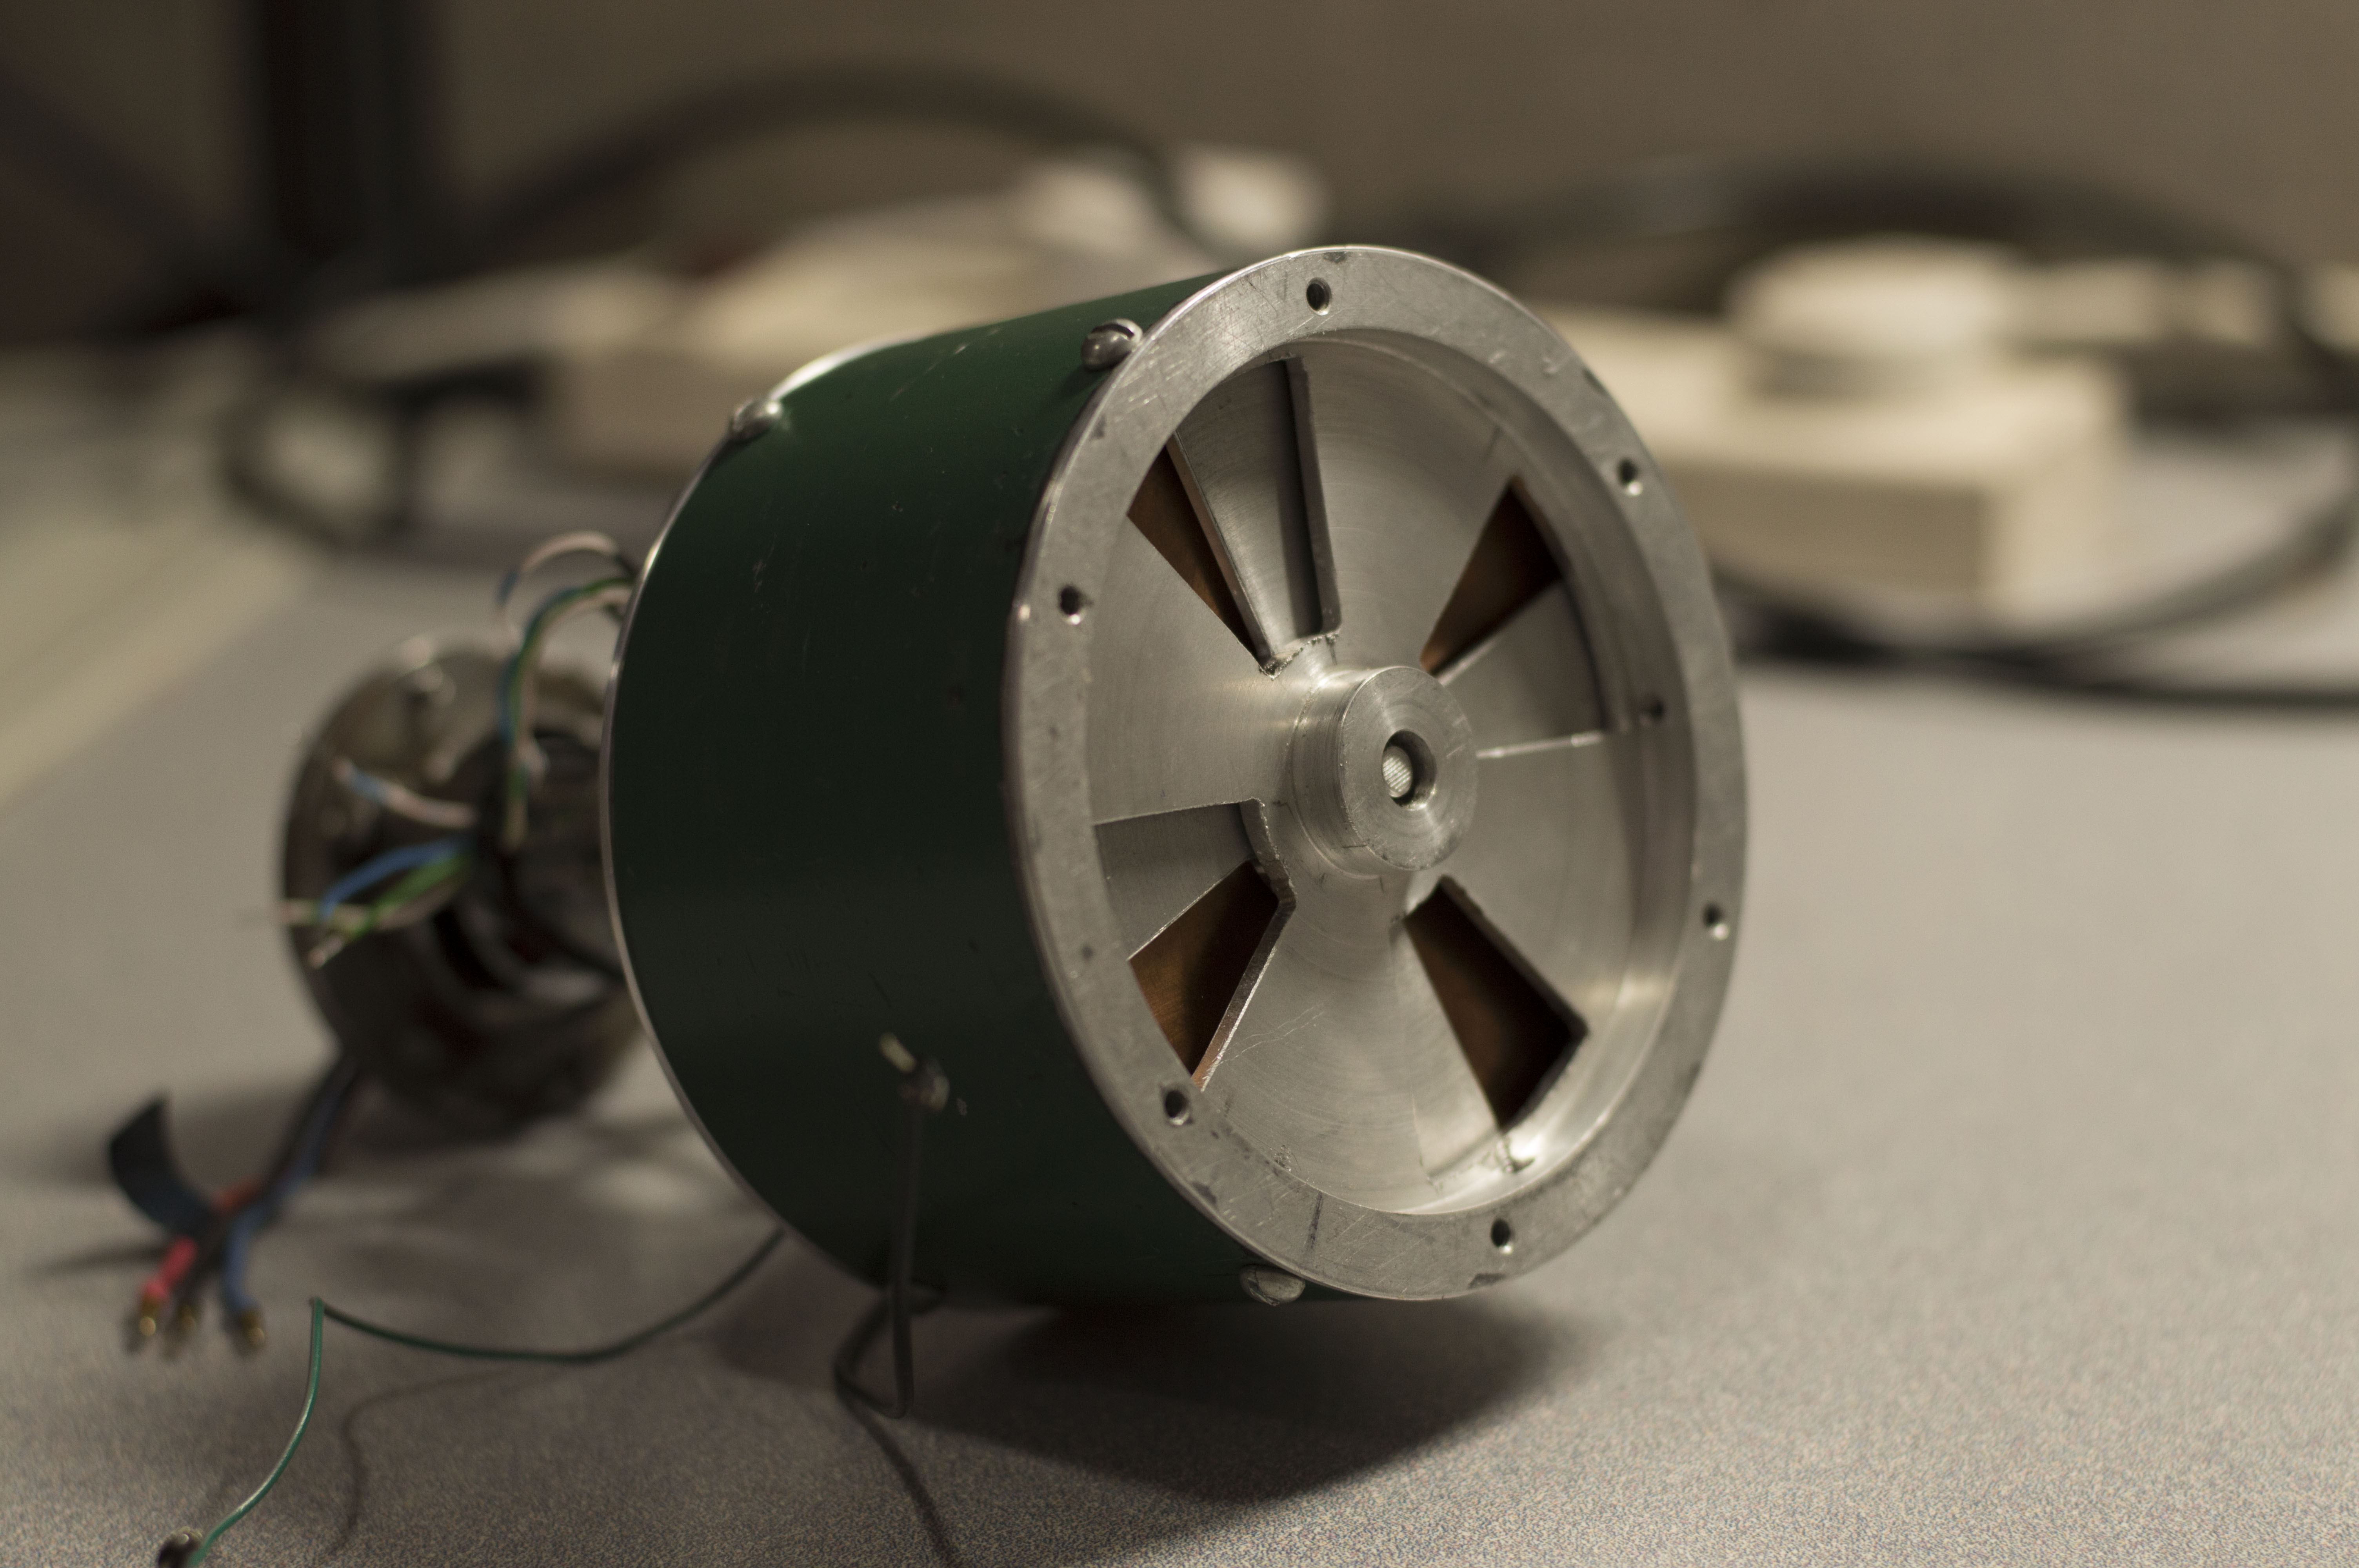
\includegraphics[width=0.80\textwidth, height = 7cm]{sensorhorizontal}
  \caption[Imagen del sensor de campo electrostático utilizado (horizontal)]{Foto del sensor en horizontal. Las aspas que pueden verse son las responsables de cubrir y descubrir la placa cargada (color cobre), que es la que se carga con la electricidad estática del ambiente.}\label{fig:sensorhorizontal}
\end{figure}

\begin{figure}[h]
  \centering
  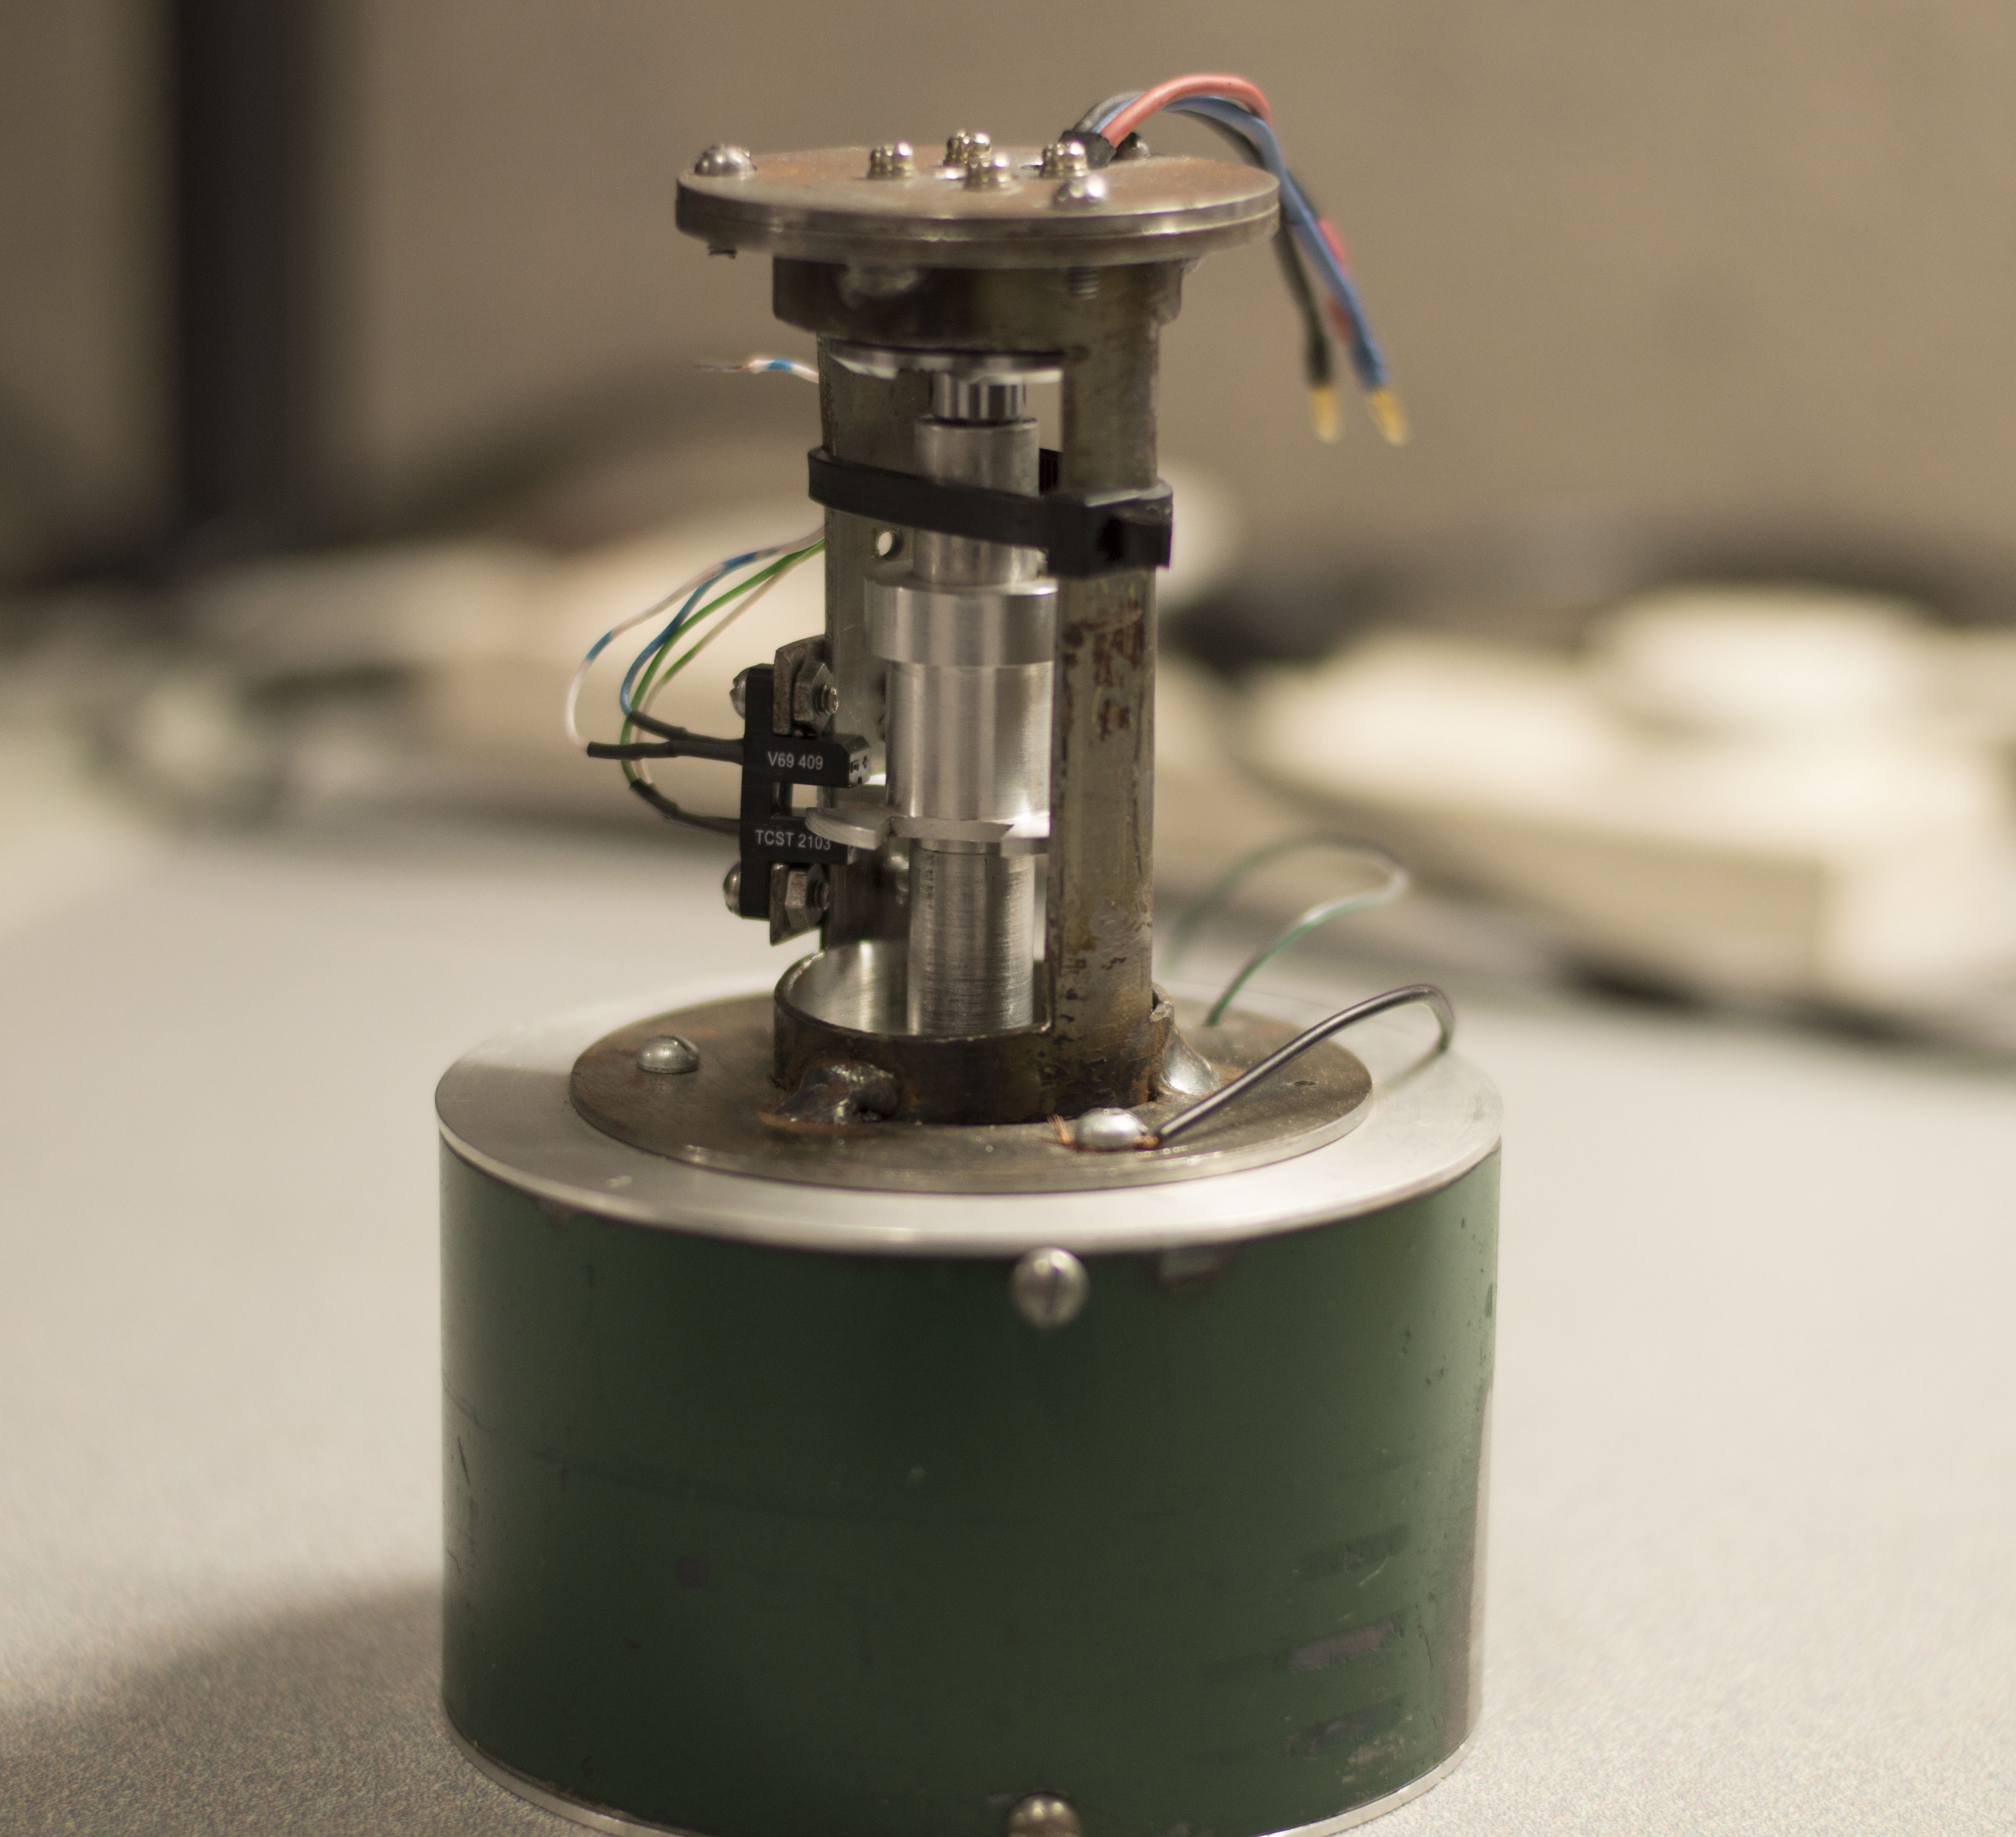
\includegraphics[width=0.80\textwidth, height = 7cm]{sensorvertical}
  \caption[Imagen del sensor de campo electrostático utilizado (vertical)]{Foto del sensor en vertical. Puede verse en el eje, el sistema de aspas y foto interruptor utilizado para medir las RPM.}\label{fig:sensorvertical}
\end{figure}

Además de las aspas que miden el campo eléctrico, en el eje del motor se encuentra un segundo grupo de aspas, pero mas pequeño; junto a estas aspas se encuentra acoplado un foto interruptor, de manera que el paso de cada aspa interrumpe el paso de luz de un extremo a otro. Si se construye el circuito requerido, ocurrirá que cuando el motor este girando, se generen pulsos cuadrados a la salida del foto interruptor, permitiendo obtener cuentas que ayudaran a la hora de controlar la velocidad del motor. Las aspas secundarias y el foto interruptor pueden verse en la figura \ref{fig:sensorvertical}

% subsection el_sensor (end)

% section introduccion (end)

\section{Requerimientos de la iteración} % (fold)
\label{it6:sec:requerimientos_de_la_iteracion}

Estos requerimientos fueron conformados teniendo en cuenta la naturaleza fisica del sensor, y las funcionalidades que ofrece la plataforma. 

\begin{itemize}
\item Se deberia utilizar la plataforma de instrumentacion para generar la señal PWM necesaria que encienda y configure el controlador del motor del sensor. [5.1]
\item Se debería poder controlar la velocidad del motor del sensor con una precision de +-50 RPM. [5.2]
\item Se debería rectificar y amplificar, con el menor ruido posible, la señal de salida del sensor, antes que ingrese al conversor de la plataforma. [5.3]
\end{itemize}


% section requerimientos_de_la_iteracion (end)

\section{Experimentación} % (fold)
\label{it6:sec:experimentacion}

El motor dentro de este sensor incluía un driver PWM. Para arrancar y dar velocidad a este motor, se utilizo, como primera instancia, una placa de desarrollo Arduino con un software hecho por Emiliano Pellicioni y Diego Gutierrez. Con el driver conectado a la placa y el programa funcionando, era posible arrancar el motor y darle una velocidad (aunque no muy constante). \\

Teniendo el motor funcionando, la teoría indica que el sensor esta midiendo campo. Para probar esto, se utilizo una regla de plástico cargada con electricidad estática y un osciloscopio conectado a la salida del sensor. Al acercar y alejar la regla de las aspas, se podía ver en la salida del osciloscopio como la onda resultante a la salida del sensor aumentaba y disminuía en amplitud. Lo que estábamos viendo, en ese momento, era una salida ``en crudo'' del sensor. Para poder convertir la señal y obtener datos coherentes, era necesario rectificar la señal. \\

El foto interruptor acoplado al eje del motor da la posibilidad de realizar un conteo de señales cuadradas que nos proporcione los datos suficientes como para realizar una medición de las vueltas por minuto del motor. Necesita de un circuito básico para funcionar. Lo construimos en una protoboard junto con todo lo necesario para hacer funcionar el motor. Con ayuda de un osciloscopio, fue posible ver los pulsos cuadrados de 5 Volts generados por el foto interruptor. Estos pulsos son los que luego servirían de entrada a un contador de eventos de la placa de instrumentación, con el objetivo de controlar la velocidad del motor. \\

ACA FALTARIA INCLUIR IMAGENES DE:

-EL OSCILOSCOPIO CON LA SALIDA DEL SENSOR MIDIENDO
-EL OSCILOSCOPIO CON LA SALIDA DEL FOTO INTERRUPTOR

% section experimentacion (end)

\section{Adaptación de la plataforma al sensor} % (fold)
\label{it6:sec:adaptacion_de_la_plataforma_al_sensor}

\subsection{Circuito de adaptación} % (fold)
\label{it6:sub:circuito_de_adaptacion}

% subsection circuito_de_adaptacion (end)

Este sensor particular requiere de ciertos requerimientos para funcionar de manera correcta:

\begin{itemize}
  \item El motor debería estar alimentado con una señal continua de 12 Voltios
  \item El driver del motor debería estar conectado a una salida de un generador de señales moduladas en ancho de pulso, con un nivel de 5 Voltios en alto y 0 Voltios en bajo.
  \item La velocidad del motor debería ser rápida y estable; priorizando la estabilidad a la velocidad.
  \item La señal de campo electrostático debería ser rectificada y amplificada previa a ser convertida a digital
\end{itemize}


Además de los requerimientos principales mencionados, fueron propuestos los siguientes requerimientos secundarios:

\begin{itemize}
  \item El diseño de la placa debería ser tal que sea acoplable y desacoplable a la placa de instrumentación.
  \item Deberia consumir lo menos posible
\end{itemize}

Para cumplir con estos requerimientos, fue necesario desarrollar funcionalidades aparte dentro del programa embebido en la plataforma de instrumentación, además de un circuito de adaptación acoplado a la misma.

% subsection requerimientos (end)
\subsubsection{Circuito de adaptación para la señal de nivel de campo} % (fold)
\label{it6:ssub:circuito_de_adaptacion_para_la_señal_de_nivel_de_campo}

La señal a la salida del sensor es alterna y de muy baja intensidad. El conversor analógico digital requiere de una señal rectificada y de un umbral mínimo para funcionar correctamente. Para esto, se diseño un circuito de adaptación de señal, que rectifica y amplifica la salida del sensor. Este circuito puede verse en la figura FIGURA.  

ACA VA EL OPERACIONAL CON EL AMPLIFICADOR Y RECTIFICADOR QUE SE PONE PARA QUE VAYA ANTES DEL CONVERSOR.. CON IMAGEN



% subsection circuito_de_adaptacion_para_la_señal_de_nivel_de_campo (end)

\subsubsection{Circuito de adaptación para la señal de pulsos del foto interruptor} % (fold)
\label{it6:ssub:circuito_de_adaptacion_para_la_señal_de_pulsos_del_fotointerruptor}


En esta configuración, el foto interruptor genera una señal de pulsos cuadrados a medida que el motor gira. Esta señal puede usarse como entrada a un contador de eventos, y de esta manera medir la velocidad de giro del motor. La figura \ref{fig:fotointerruptorcircuitotipico} muestra el circuito implementado para este fin. 

\begin{figure}[h]
  \centering
  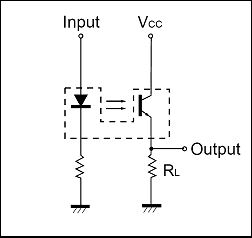
\includegraphics[width=0.50\textwidth, height = 5cm]{fotointerruptorcircuitotipico}
  \caption{Circuito utilizado para el fotointerruptor}\label{fig:fotointerruptorcircuitotipico}
\end{figure}

En esta disposición, cuando el foto sensor esta iluminado, hay 5 Volts en la salida; de lo contrario 0 Volts. Esto hace que cuando el motor gira, las aspas van a tapar y destapar la entrada de luz al foto sensor generando una onda cuadrada a la salida del circuito, cuya frecuencia depende de la velocidad del motor. Dentro del software de la plataforma de instrumentación, se utilizo uno de los contadores de eventos disponibles para obtener las cuentas del foto interruptor y medir la velocidad del motor. Con esta información, se modifica el ancho de pulso de la señal PWM a la entrada del driver del motor. Corrigiendo así la velocidad, para mantenerla lo mas estable posible. 

% subsection circuito_de_adaptacion_para_la_señal_de_pulsos_del_fotointerruptor (end)

\subsubsection{Circuito de alimentación} % (fold)
\label{it6:ssub:circuito_de_alimentacion}

La placa de instrumentación esta diseñada para estar siempre encendida. Al no consumir mucho, no trae problemas de consumo o temperatura. Pero habiendo hecho esta adaptación, era necesario tener en cuenta el consumo del motor mientras esta encendido pero sin girar. Para ahorrar consumo, propusimos agregar un control de encendido y apagado del sensor, utilizando uno de los pines GPIO del microcontrolador. \\

La figura PONER FIGURA DEL CIRCUITO muestra el circuito que prepara la señal del microcontrolador que controla el encendido y apagado del motor. Utilizamos un relé, un opto acoplador, un transistor, un diodo y resistencias. El opto acoplador sirve para aislar apáticamente el circuito lógico del motor con el circuito de 12 V. El relé electromecánico conmuta la conductividad entre el motor y masa, de manera que en un estado del relé el motor esta prendido, y en el otro esta apagado. Utilizamos un transistor porque los 5V a la salida del opto acoplador no eran suficientes para la tensión de switching del relé.

% subsection circuito_de_alimentacion (end)

\subsubsection{Señal modulada en ancho de pulso para el adaptador del motor} % (fold)
\label{it6:ssub:señal_modulada_en_ancho_de_pulso_para_el_adaptador_del_motor}

% aca en realidad no hicimos nada porque lo unico que hay es el cable de salida del pwm que viene de la placa y se conecta de pecho al driver.. pero bueno explicar eso.. y explicar tambnein que pasamos desde el arduino que hacia todo por interrupciones al pwm de la placa que lo hace todo por HW y funciona mucho mejor. aunque no explicar como funciona el programa porque eso va despues

El motor dentro de la estructura que conforma el motor tiene un modulo adaptador programable que funciona como interfaz, haciendo que una señal modulada en ancho de pulso se convierta en la velocidad de giro del motor, así como también en distintas configuraciones. Los distintos anchos de pulso son códigos que representan distintos modos para el driver. En el manual, especifica las distintas configuraciones disponibles y como establecerlas utilizando distintas señales moduladas en ancho de pulso. Tanto en el proceso de configuración como en el funcionamiento normal, el driver emite sonidos en distintos tonos que dan información sobre el estado en cada momento.

Para una respuesta estable del sensor, era importante que las aspas giren a una velocidad alta y constante. Alrededor de los 4000 RPM, priorizando la estabilidad a la velocidad. Dentro del programa de la plataforma de instrumentación, existen rutinas que establecen el driver automaticamente en el modo requerido por nuestro sistema. Estas rutinas utilizan un modulo del microcontrolador denominado PCA, que incluye, en uno de sus modos, un generador de señal modulada en pulsos. Cuando el motor esta en funcionamiento, el mismo programa se encarga de estabilizar su velocidad con las funciones descritas en la sección \ref{it6:sec:software_de_adaptacion}


% subsection circuito_de_adaptacion_para_la_señal_modulada_en_ancho_de_pulso_para_el_driver_del_motor (end)

\subsubsection{Circuito final} % (fold)
\label{it6:ssub:circuito_final}

En las secciones anteriores, describimos por separado cada una de las partes del circuito de adaptación para el sensor de campo. La figura FIGURA muestra el despliegue de componentes del circuito final. Este diseño se imprimió en un PCB para acoplar a la plataforma de instrumentación. El circuito impreso y acoplado se muestra en la figura FIGURA.


% subsection circuito_final (end)

% section implementacion_de_una_placa_de_adaptacion_para_el_sensor_de_campo (end)


\subsection{Software de adaptación} % (fold)
\label{it6:sec:software_de_adaptacion}


El circuito de adaptación, prepara las señales de entrada y salida necesarias para el funcionamiento correcto del sensor. Dentro de la placa de instrumentación, desarrollamos funcionalidades anexas al software principal para trabajar estas señales.
Realizamos un modulo aparte llamado ``sensor\_CE.c'', cuyas funciones están desarrolladas de manera especifica para este sensor. Estas funciones incluyen:

\begin{itemize}
  \item Dar arranque y parada al motor
  \item Controlar la velocidad del motor.
\end{itemize}

La medición de campo no es parte del software de adaptación, dado que se realiza utilizando funciones del modulo ``conversor''. La señal proveniente del circuito de adaptación que corresponde a la telemetría proveniente del sensor, se conecta a uno de los pines de entrada del conversor analógico-digital. \\

La figura \ref{fig:diagramabloquessensor} muestra el diagrama de bloques de la adaptación del software a la plataforma de instrumentación.

\begin{figure}[h]
  \centering
  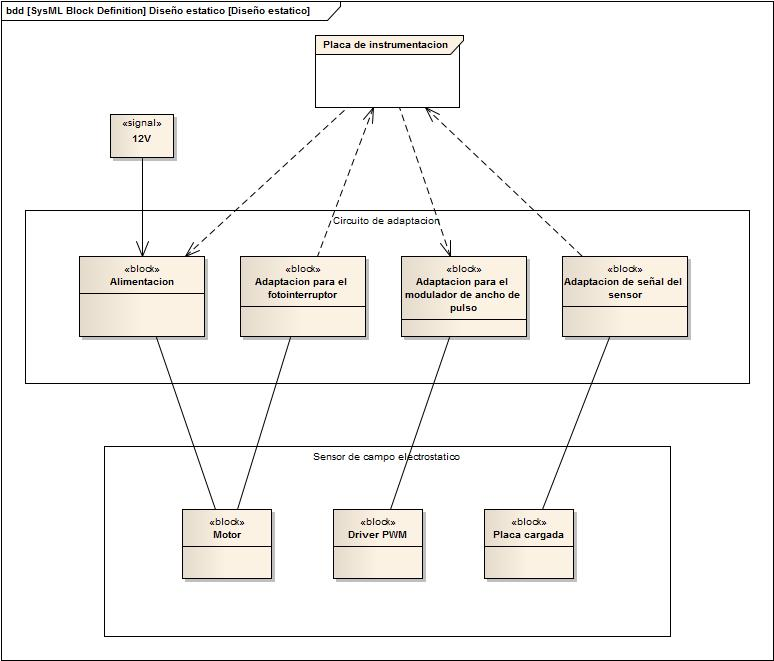
\includegraphics[width=0.80\textwidth, height = 7cm]{diagramabloquessensor}
  \caption{Diagrama de bloques físicos del sistema de adaptación del sensor}\label{fig:diagramabloquessensor}
\end{figure}

\subsubsection{Arranque y parada} % (fold)
\label{it6:ssub:arranque_y_parada}

El motor esta controlado por un driver PWM que traduce señales moduladas en ancho de pulso en la corriente trifásica que da giro al motor. Para dar arranque al motor, es necesario seguir una serie de pasos que dependen del modo configurado en el driver. Para dar fin al giro del motor, simplemente hay que apagar la señal PWM. \\

Para este caso particular, es necesario utilizar un único modo de configuración, ya que se necesita que el motor gire a una única velocidad, lo mas estable posible. El modo de configuración esta establecido aunque el driver esta apagado. En caso de necesitar reconfigurarlo, existen funciones dentro del software de adaptación que lo permiten. \\

Si el driver esta configurado correctamente y esta alimentado a 12 Voltios, es necesario activar la secuencia de arranque para que comience a girar. Esta secuencia de arranque consiste en 3 señales de distintos anchos de pulso separadas por intervalos de un segundo. Luego de esta secuencia, se establece el ancho de pulso que da la velocidad estable al motor, configurada en este caso para 4000 RPM. \\

Una vez que el motor alcanzo su velocidad estable, se activa el control de velocidad, para evitar que se desestabilice. 

\begin{figure}[h]
  \centering
  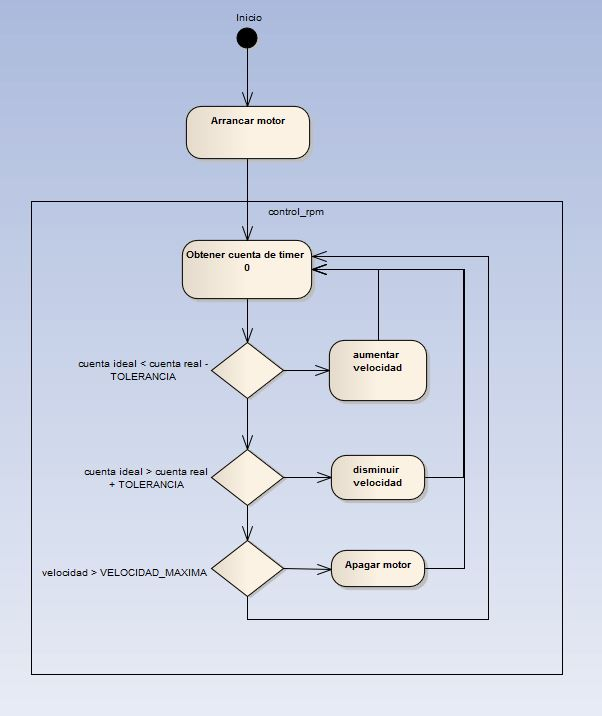
\includegraphics[width=0.80\textwidth, height = 7cm]{diagramaactividadescontrolvelocidad}
  \caption{Diagrama de actividades para el control de arranque del motor}\label{fig:diagramaactividadesarrancarmotor}
\end{figure}

% subsubsection arranque_y_parada (end)

\subsubsection{Control de velocidad} % (fold)
\label{it6:ssub:control_de_velocidad}

La velocidad de giro del motor debería ser rápida y constante para un mejor funcionamiento del sensor, priorizando estabilidad a velocidad. Para lograr esto, utilizamos el foto interruptor acoplado al sensor, como generador de pulsos cuadrados. Estos pulsos se usan como entrada a uno de los contadores de eventos de la plataforma de instrumentación. Con el valor de esta cuenta, es posible calcular la velocidad del motor en tiempo real, con una precisión de unos 30 milisegundos por medición. \\

La estabilidad en en la velocidad de giro del motor se alcanzo mediante un control básico de velocidad, hecho por software. Estableciendo una base de tiempo con uno de los timer del microcontrolador, se cuenta la cantidad de eventos sobre esa base de tiempo, la cantidad de cuentas entonces, da la velocidad. Una velocidad ``estable'' esta establecida en una variable fija, y se corresponde a una cantidad fija de eventos en la misma base de tiempo. Comparando la cantidad de eventos medidos sobre la base de tiempo con la cantidad de eventos que corresponden a la velocidad estable, se sabe si el motor esta girando demasiado rápido, o demasiado lento. Con esta información, se ajusta la velocidad del motor para acelerarlo o desacelerarlo, modificando el ancho de pulso del modulo PCA conectado al driver PWM del motor. Una descripción gráfica de este proceso se ilustra en la figura \ref{fig:diagramaactividadescontrolvelocidad}

\begin{figure}[h]
  \centering
  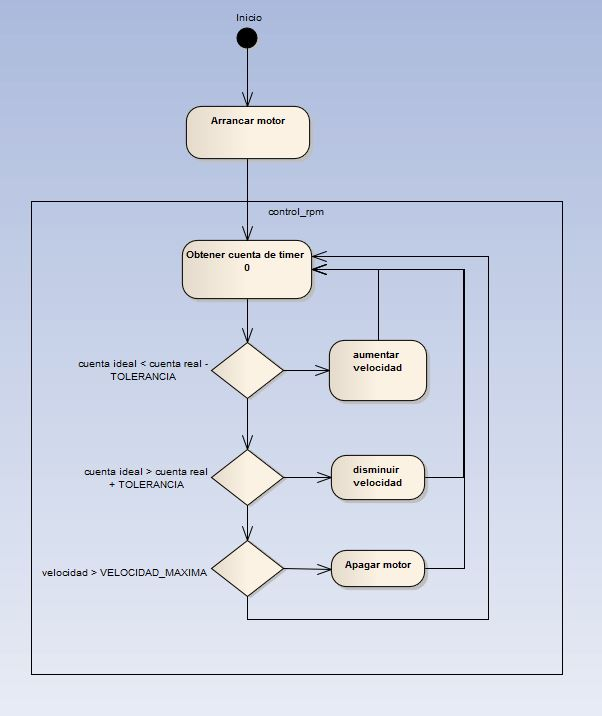
\includegraphics[width=0.80\textwidth, height = 7cm]{diagramaactividadescontrolvelocidad}
  \caption{Diagrama de actividades para el control de velocidad del motor}\label{fig:diagramaactividadescontrolvelocidad}
\end{figure}

% subsubsection control_de_velocidad (end)



% section funcionalidades_desarrolladas_dentro_del_software_de_la_placa_de_instrumentacion_para_trabajar_junto_con_el_sensor (end)

\section{Pruebas} % (fold)
\label{it6:sec:pruebas}

\begin{table}[h]
\centering
\caption{Test de sistema 1: Comprobación de estabilidad del motor}
\label{it6:tab:testsistema1}
\begin{tabular}{p{2cm} p{9cm}}
\multicolumn{2}{c}{\cellcolor[HTML]{68CBD0}{\color[HTML]{000000} Prueba de sistema}} \\
Prueba \#        & 1 \\
\hline
Nombre           & Comprobación de estabilidad del motor \\                     
\hline
Requerimiento    & 5.2  \\
\hline
Descripción      & Se arranca el motor del sensor y se lo configura en la velocidad de medición. Verificando que se se estabilice en esa velocidad\\
\hline
Pre-condiciones  & \tabitem Plataforma de instrumentación encendida y disponible para configurar  \\
                 & \tabitem Computadora conectada al sistema mediante cable serial RS-232 \\
                 & \tabitem Lector de canal serial abierto en la computadora  \\
                 & \tabitem Circuito de adaptación del sensor alimentado y correctamente conectado a la plataforma \\
                 & \tabitem Velocidad estable de 3000 RPM configurada en el código de las funciones del sensor, dentro de la plataforma. \\
                 & \tabitem Impresión en pantalla de velocidad del motor incluida en la función de control del mismo, dentro del código de la plataforma. \\
\hline

Post-condiciones & La velocidad del motor debería ser estable.  \\
\hline
Secuencia  & \tabitem Ingresamos el comando ``PWM'' en la interfaz MML \\
           & \tabitem Esperamos que el motor finalice la secuencia de arranque. \\
           & \tabitem Una vez que el motor anduvo durante 10 segundos seguidos, se le da parada mediante el comando ``NTP'' \\

\hline
Resultados       & La velocidad fue medianamente estable, con algunas perturbaciones no periódicas, en la velocidad configurada (3000 RPM). La influencia de las perturbaciones en la velocidad sobre las mediciones de campo, fue analizada en la prueba de sistema 2.
\end{tabular}
\end{table}

\begin{table}[h]
\centering
\caption{Test de sistema 2: Medición de campo}
\label{it6:tab:testsistema2}
\begin{tabular}{p{2cm} p{9cm}}
\multicolumn{2}{c}{\cellcolor[HTML]{68CBD0}{\color[HTML]{000000} Prueba de sistema}} \\
Prueba \#        & 1 \\
\hline
Nombre           & Medición de campo \\                     
\hline
Requerimiento    & 5.1 \\
\hline
Descripción      & Se arranca el motor del sensor y se mide campo, esperando obtener una medición estable, que además cambie de valor a medida que se perturba el campo eléctrico cerca del sensor. \\
\hline
Pre-condiciones  & \tabitem Sistema configurado con el pin 0 en modo canal unico, con un intervalo de 1 \\
                 & \tabitem Salida correspondiente a la señal del sensor (rectificada y amplificada por el circuito de adaptación) conectada al pin configurado en el punto anterior. \\
                 & \tabitem Plataforma de instrumentación encendida y disponible para configurar  \\
                 & \tabitem Computadora conectada al sistema mediante cable serial RS-232 \\
                 & \tabitem Lector de canal serial abierto en la computadora  \\
                 & \tabitem Circuito de adaptación del sensor alimentado y correctamente conectado a la plataforma \\
                 & \tabitem Motor del sensor encendido y girando a una velocidad estable \\
                 & \tabitem Plataforma de instrumentación midiendo en modo de conversiones continuas \\
\hline

Post-condiciones & \tabitem El campo eléctrico medido debería ser estable, a pesar de las variaciones en la velocidad del motor registradas en la prueba de sistema 1. \\
\hline
Secuencia  & \tabitem Leímos los datos de salida de las conversiones continuas y esperamos a que el resultado sea estable. \\
           & \tabitem Con un dispositivo cargado de electricidad estática, perturbamos el campo eléctrico cercano a las aspas del sensor. \\

\hline
Resultados       & La medición logro estabilizarse, y la perturbación del campo eléctrico se correspondía con los datos impresos en la interfaz. Las variaciones en la velocidad, producto de fallas en la estabilización, no hicieron que la medición de campo variara significativamente.
\end{tabular}
\end{table}

\begin{table}[h]
\centering
\caption{Test de sistema 3: Rectificación y amplificación}
\label{it6:tab:testsistema3}
\begin{tabular}{p{2cm} p{9cm}}
\multicolumn{2}{c}{\cellcolor[HTML]{68CBD0}{\color[HTML]{000000} Prueba de sistema}} \\
Prueba \#        & 1 \\
\hline
Nombre           & Rectificación y amplificación \\                     
\hline
Requerimiento    & 5.3  \\
\hline
Descripción      & Con el sensor encendido y girando a una velocidad estable, se mide, con uso de un osciloscopio, la señal a la salida del sensor, a la salida de la etapa de amplificación, y a la salida de la etapa de rectificación, para luego analizar los resultados.\\
\hline
Pre-condiciones  & \tabitem Osciloscopio encendido \\
                 & \tabitem Salida correspondiente a la señal del sensor (rectificada y amplificada por el circuito de adaptación) conectada a un borne positivo del osciloscopio. \\
                 & \tabitem Salida correspondiente a la señal del sensor a la salida del rectificador (ya amplificada) , conectada a otro borne positivo del osciloscopio  \\
                 & \tabitem Salida correspondiente a la señal del sensor a la salida del amplificador, conectada a otro borne positivo del osciloscopio  \\
                 & \tabitem Circuito de adaptación del sensor alimentado \\
                 & \tabitem Motor del sensor encendido y girando a una velocidad estable \\
\hline

Post-condiciones & \tabitem La señal a la salida de la etapa de amplificación debería tener mas amplitud que a la salida del sensor \\
                 & \tabitem La señal a la salida de la etapa de rectificación no debería tener valores negativos.\\
\hline
Secuencia  & \tabitem Con un dispositivo cargado de electricidad estática, perturbamos el campo eléctrico cercano a las aspas del sensor. \\
           & \tabitem Analizamos la salida del osciloscopio \\

\hline
Resultados       & Las salidas del osciloscopio respondieron como era esperado a las perturbaciones.
\end{tabular}
\end{table}

% section pruebas (end)


\section{Conclusiones} % (fold)
\label{it6:sec:conclusiones}

Nuestro objetivo, con la construcción de esta adaptación, fue obtener una prueba de campo para verificar el funcionamiento de la plataforma en un contexto real.

Los avances de esta iteración permitieron controlar las variables del sensor que eran necesarias para el correcto funcionamiento del mismo. El arranque y giro del motor, la estabilidad del mismo, y el procesamiento de la señal de la placa sensitiva, son funciones que fueron provistas por el software agregado a la plataforma y por el hardware en el circuito de adaptación. 

La iteración siguiente sera destinada a la construcción de un sistema embebido que tome los datos de telemetría y controle la plataforma. Además de esto, agregaremos funcionalidades especificas, en este sistema embebido, para la adaptación hecha en esta iteración. 

% section conclusiones (end)

% chapter iteracion_6 (end)